\section{Photonic reservoir computer with wavelength division multiplexed neurons}

\begin{frame}{Wavelength division multiplexing of the neurons}
	\begin{figure}
		\centering
		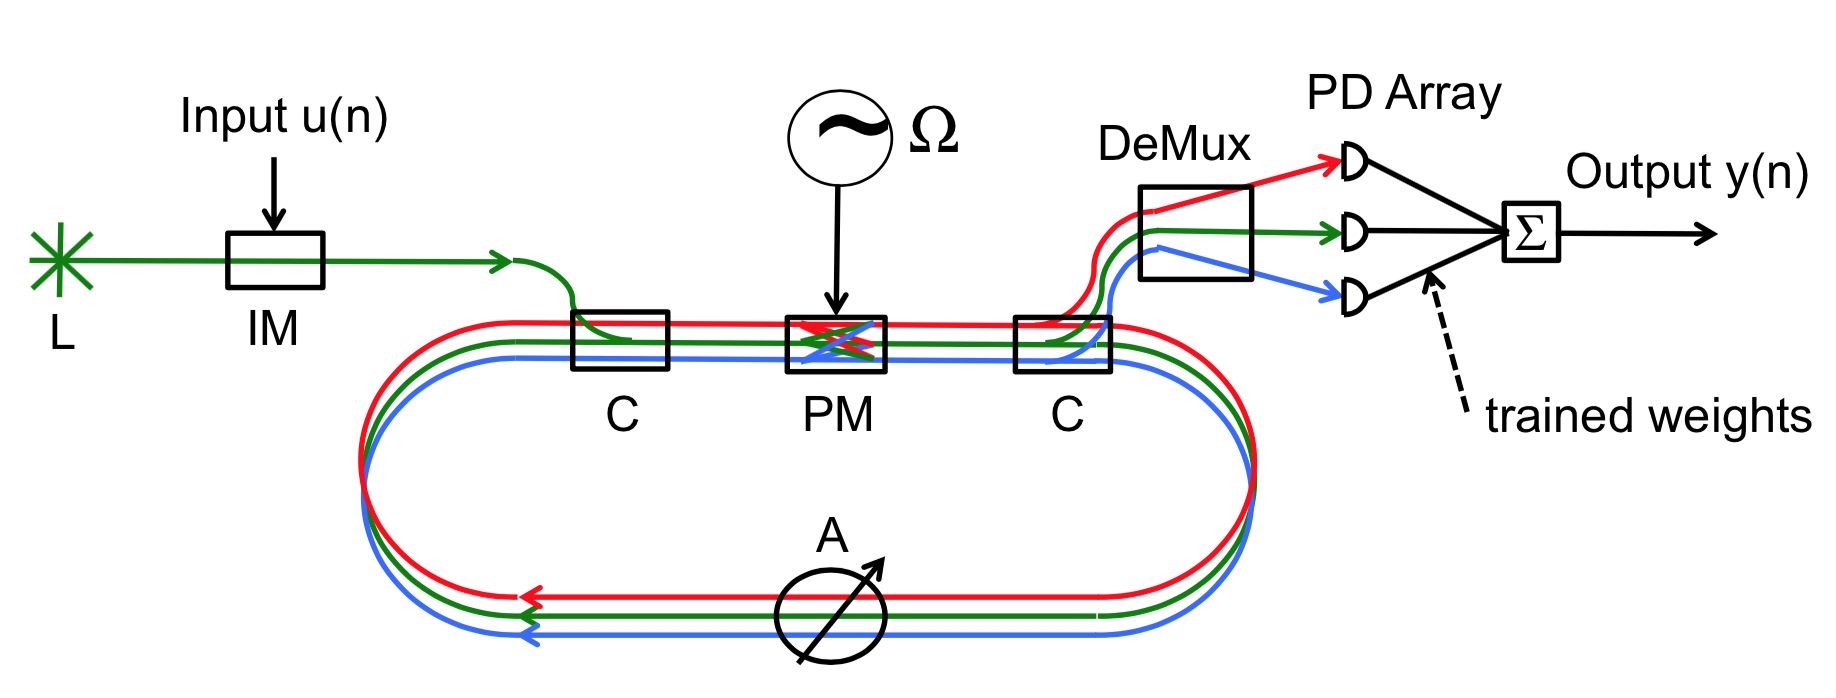
\includegraphics[width=.7\textwidth]{wdm_rc_principle.png}
		\caption{\cite{AkroutAkram2016Pprc}}
	\end{figure}
	\begin{itemize}
		\item \textcolor{ForestGreen}{Input} : monochromatic laser modulated in amplitude $\rightarrow u(n)$
		\item \alert{Optical cavity stabilisation with intra-cavity phase modulation}
		\item Output : wavelength demultiplexing and linear combination
	\end{itemize}
\end{frame}

\begin{frame}{Frequency coupling of the neurons - phase modulator}
	\begin{equation*}
		E e^{i\omega t} \overset{\color{ForestGreen} \Omega \color{black}}{\longrightarrow} E e^{i\omega t} e^{i \color{orange} m \color{black} \sin{(\color{ForestGreen} \Omega \color{black} t)}} = E \sum_{n=-\infty}^{\infty} \color{blue}J_n\color{black}(\color{orange}m\color{black}) e^{i(\omega+n \color{ForestGreen} \Omega \color{black})t}
	\end{equation*}
	\begin{itemize}
		\item $\color{blue}J_n\color{black}$ : Bessel function of order $n$
		\item $\color{orange}m\color{black}$ : modulation depth
		\item $\color{ForestGreen} \Omega \color{black}$ : modulation frequency $\approx \SI{20}{\giga\hertz}$
	\end{itemize}
	\begin{figure}
		\centering
		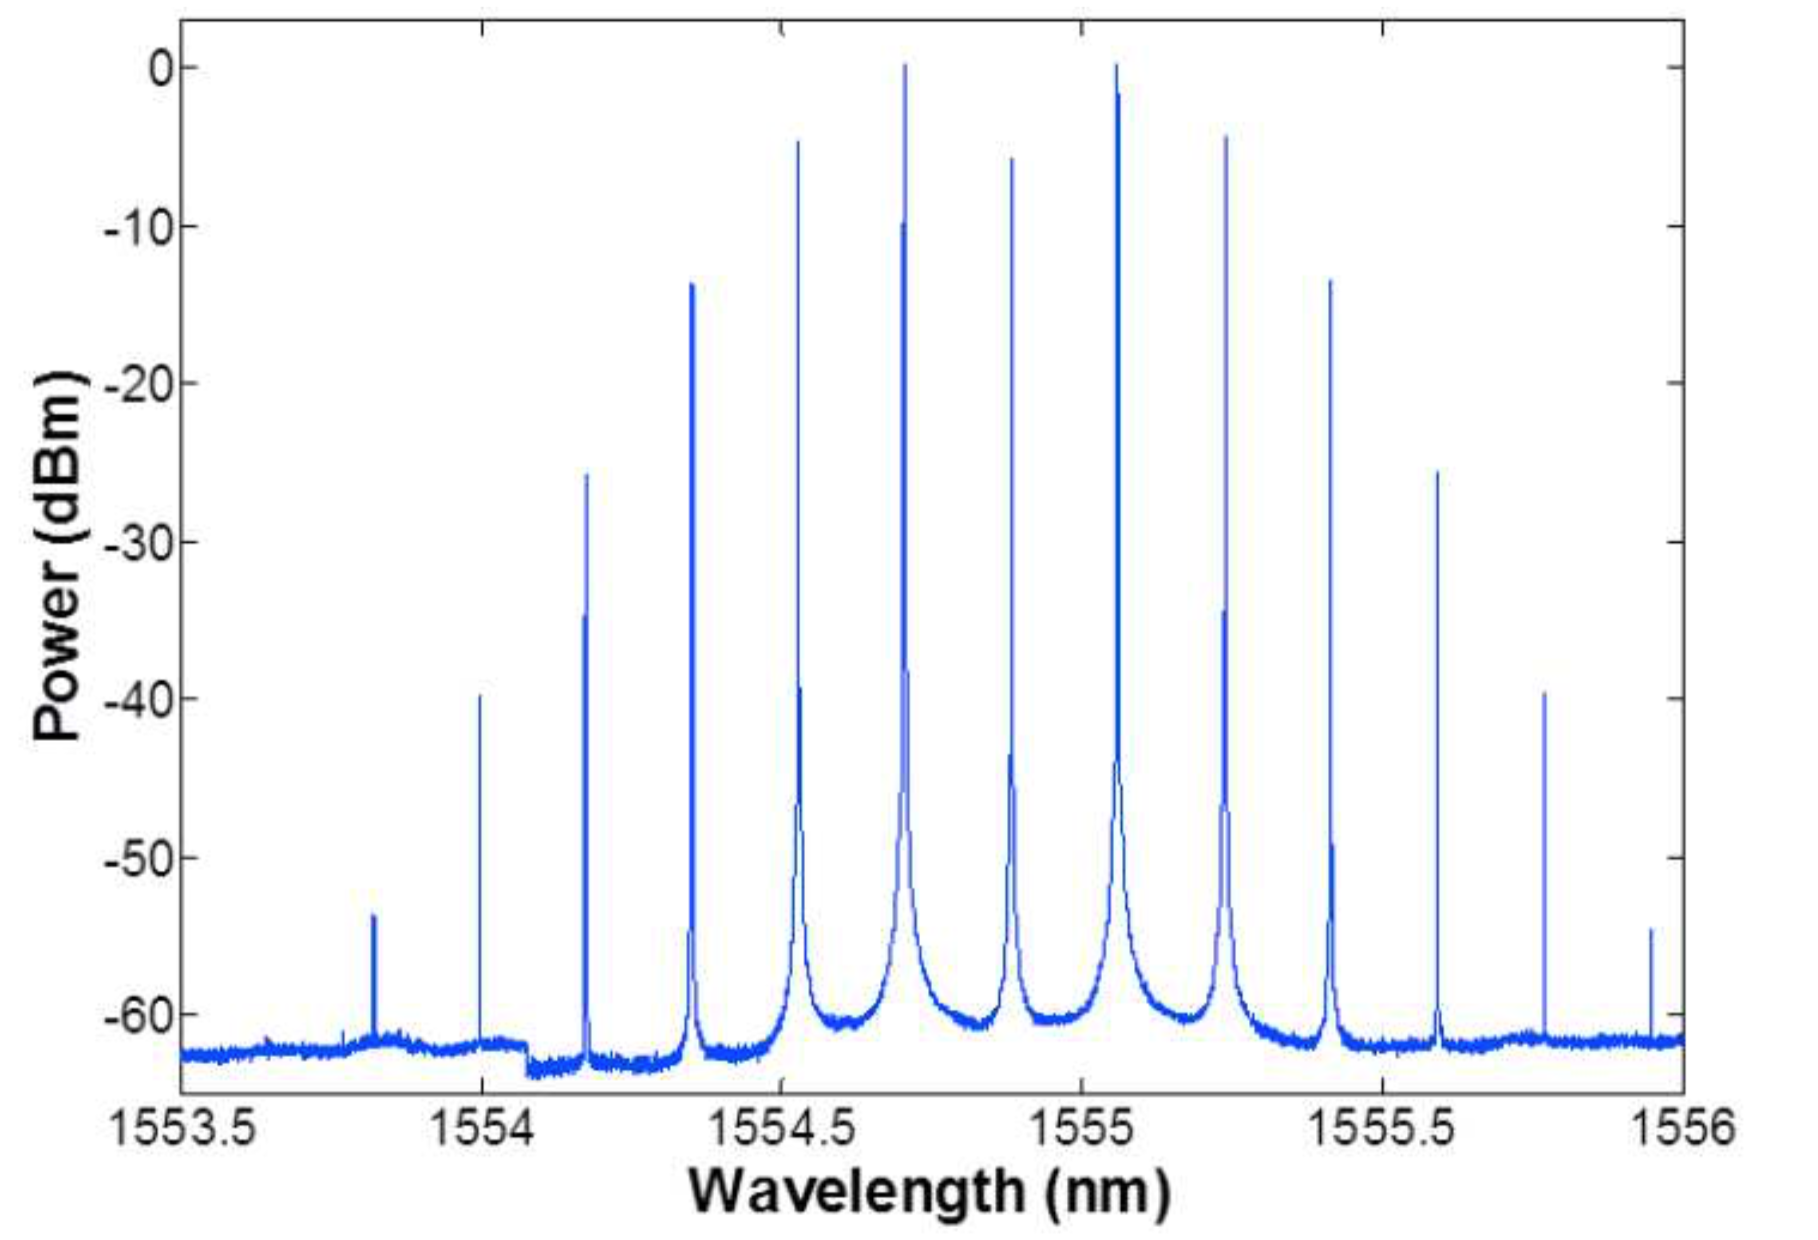
\includegraphics[width=.4\textwidth]{power-in-neurons.png}
	\end{figure}
	\centering
	$\color{red}\hookrightarrow$ \alert{Only 13 neurons !}
\end{frame}

\begin{frame}{Cavity transfer function \textbf{without} phase modulation}
	\begin{columns}
		\begin{column}{.5\textwidth}
			\begin{figure}
				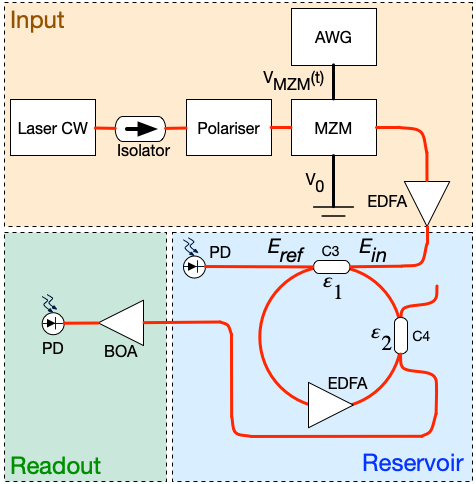
\includegraphics[width=\textwidth]{exp-setup1.png}
			\end{figure}
		\end{column}%
		\begin{column}{.5\textwidth}
			\begin{itemize}
				\item Reflectivity :
				\begin{equation*}
					\mathcal{R}(\omega) = 1-\frac{1}{1+\mathcal{F}\sin^2{(\frac{\omega}{\text{FSR}})}}
				\end{equation*}
			\end{itemize}
			\begin{figure}
				\centering
				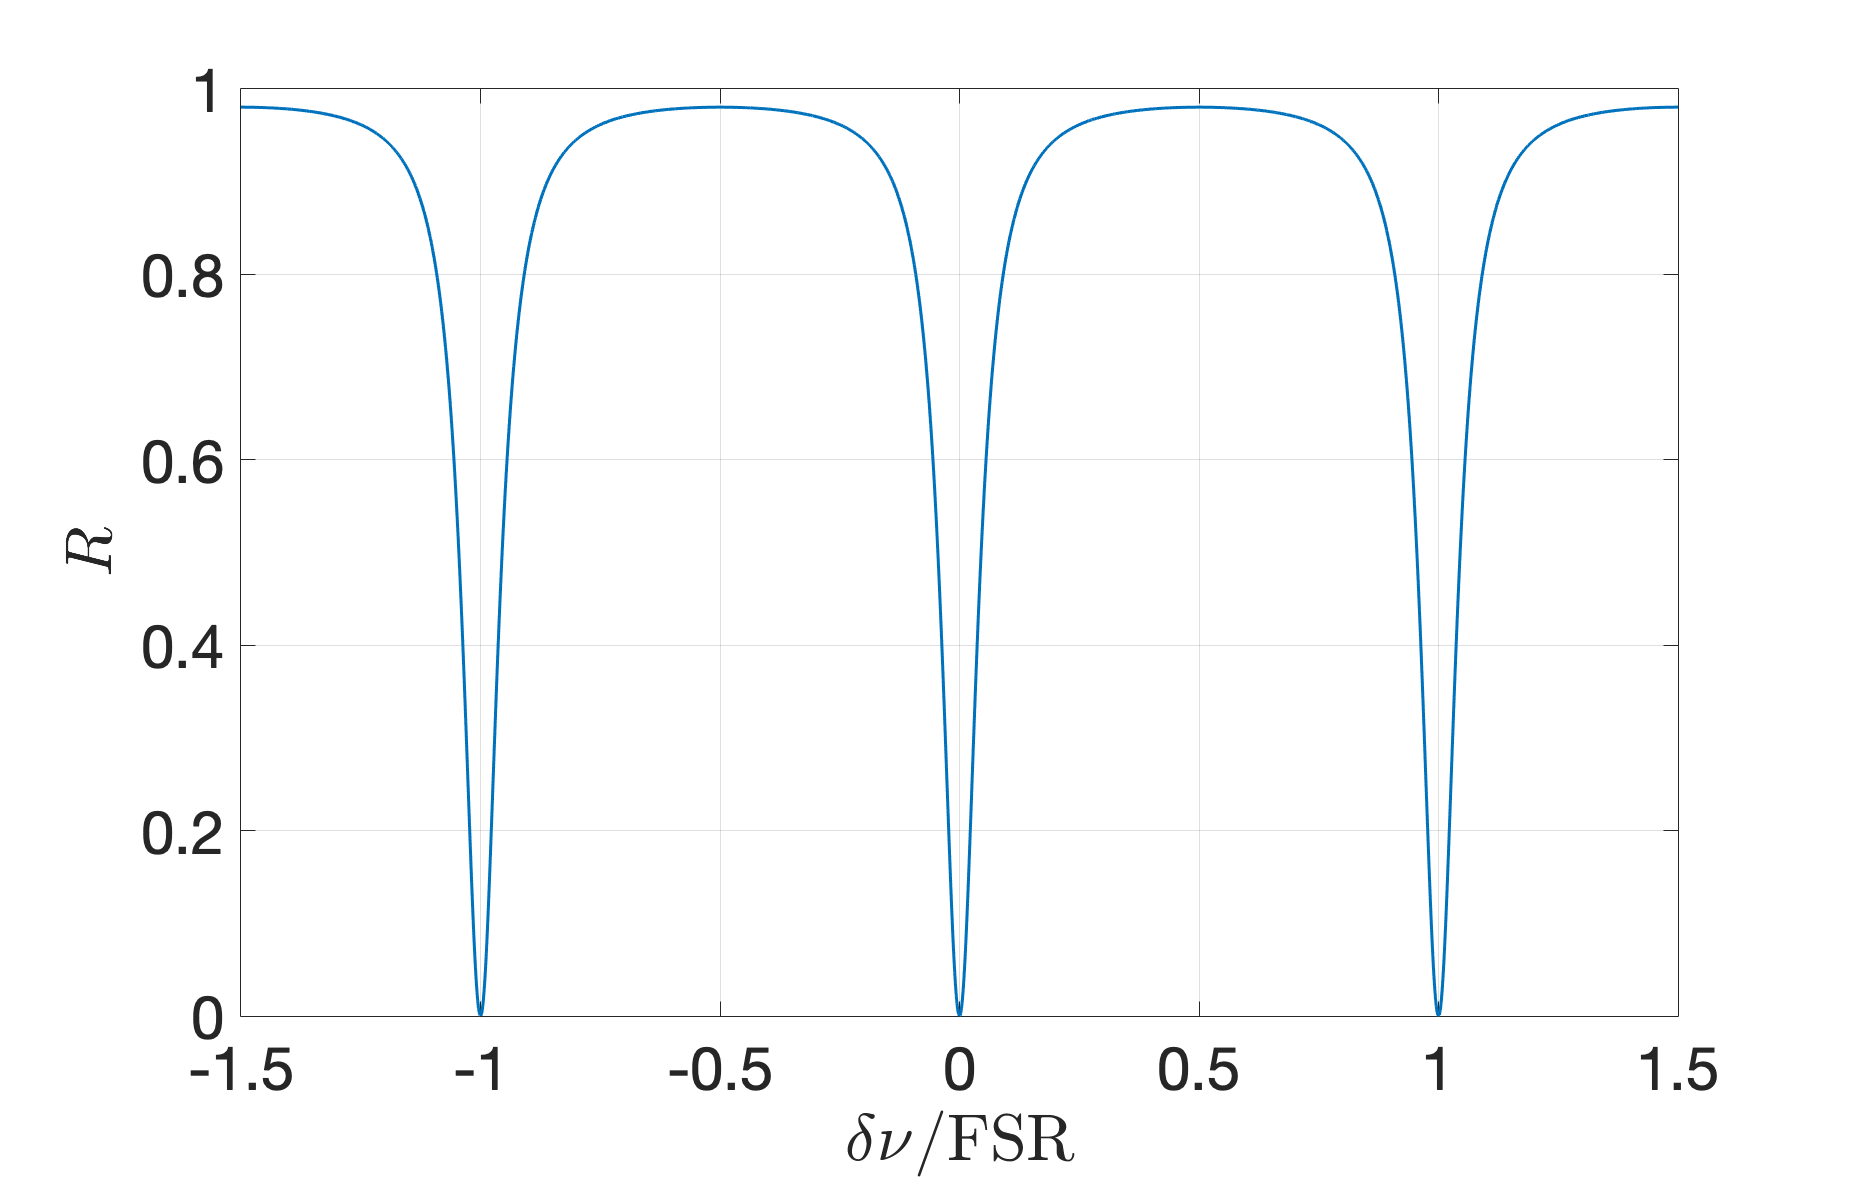
\includegraphics[width=\textwidth]{fp-ref-tf.png}
			\end{figure}
			\centering
			$\color{red}\hookrightarrow$ \alert{Symmetric}
		\end{column}
	\end{columns}
\end{frame}

\begin{frame}{Cavity transfer function \textbf{with} phase modulation}
	\begin{figure}
		\centering
		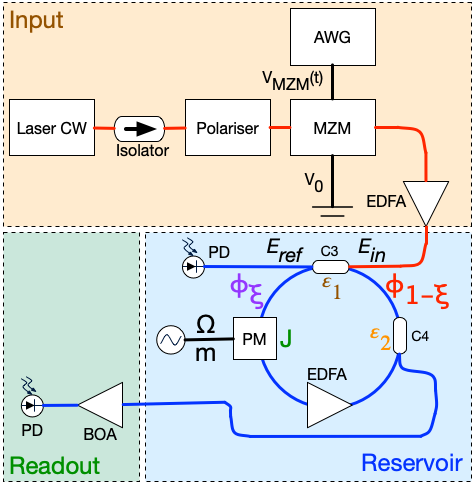
\includegraphics[width=.43\textwidth]{exp-setup2.png}
	\end{figure}
	\begin{alertblock}{Transfer matrix}
		\begin{equation*}
			\mathbf{R} = \color{brown} \epsilon_1 \color{black} \mathbf{I} - (1-\color{brown} \epsilon_1 \color{black}^2) \color{orange} \epsilon_2 \color{black} e^{-\gamma L} \left( \mathbf{I} - \color{brown} \epsilon_1 \color{black} \color{orange} \epsilon_2 \color{black} e^{- \gamma L} \color{red} \Phi_{1-\xi} \color{black} \color{ForestGreen} \mathbf{J} \color{black} \color{RoyalPurple} \Phi_\xi \color{black} \right)^{-1} \color{red} \Phi_{1-\xi} \color{black} \color{ForestGreen} \mathbf{J} \color{black} \color{RoyalPurple} \Phi_\xi \color{black}
		\end{equation*}
	\end{alertblock}
\end{frame}

\begin{frame}{Cavity transfer function \textbf{with} phase modulation}
	\begin{equation*}
		\mathcal{R}(\omega) = \sum_{n=-\eta}^\eta |R_{n,0} (\omega) |^2
	\end{equation*}
	\begin{columns}
		\begin{column}{.5\textwidth}
			\begin{figure}
				\centering
				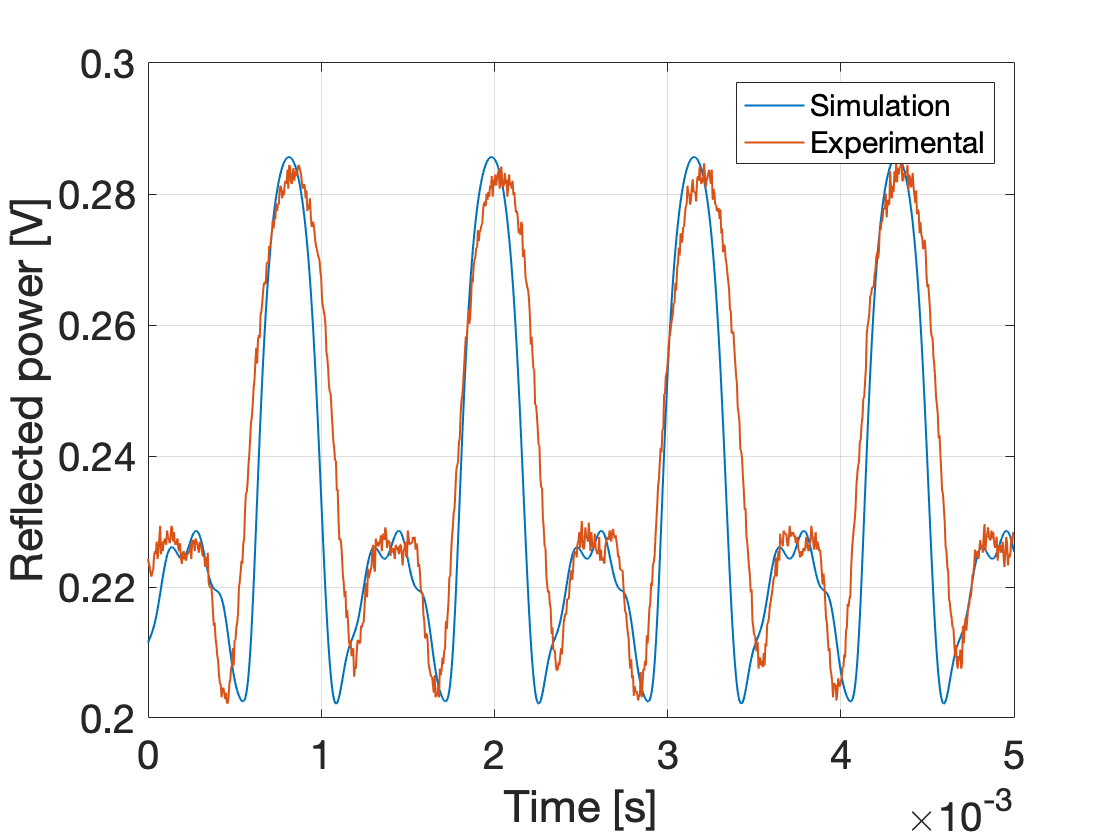
\includegraphics[width=\textwidth]{tf_0.png}
			\end{figure}	
		\end{column}%
		\begin{column}{.5\textwidth}
			\begin{figure}
				\centering
				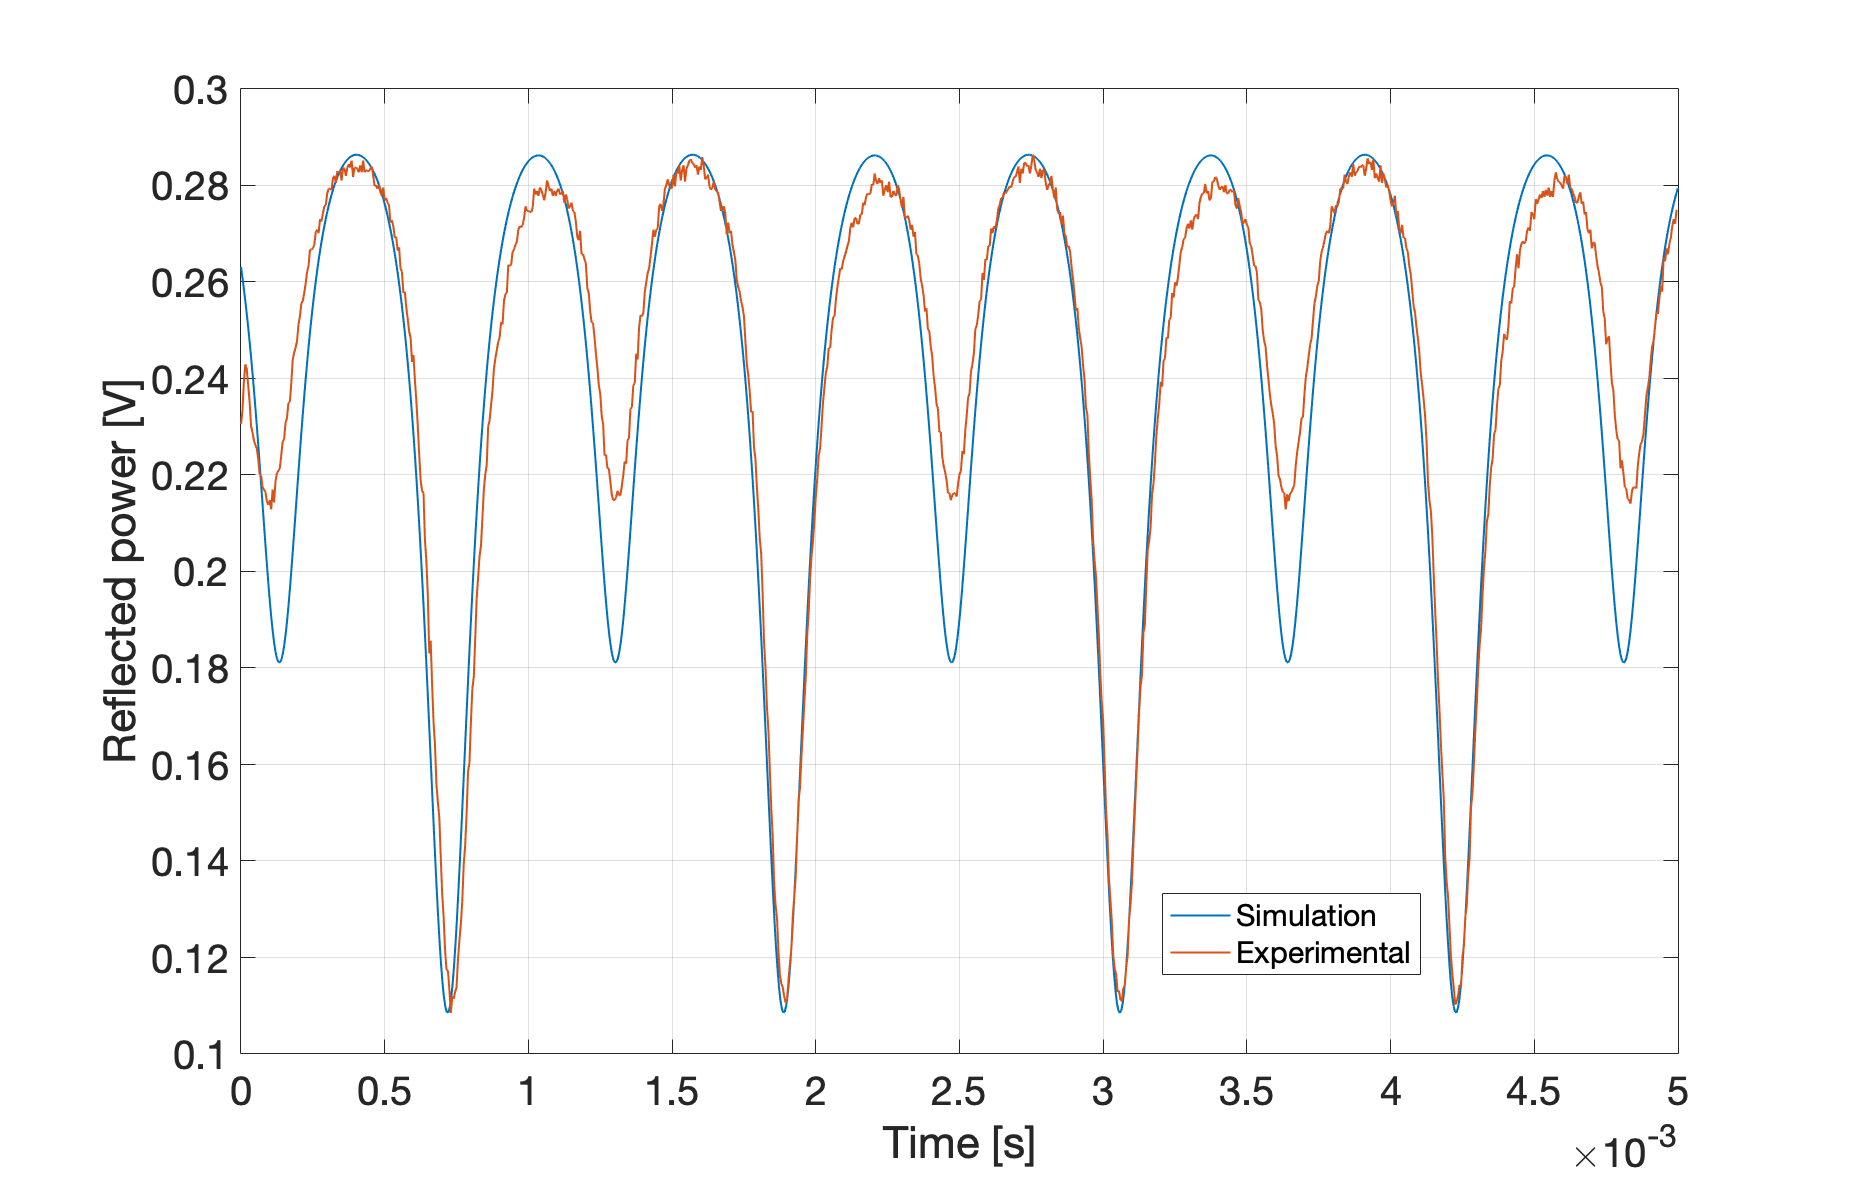
\includegraphics[width=\textwidth]{tf_50.png}
			\end{figure}	
		\end{column}
	\end{columns}
	\vspace{1em}
	\centering
	$\color{red} \hookrightarrow $ \alert{More complex} $\color{red} \Rightarrow$ \alert{hard to stabilise !}	
\end{frame}







